% v2-acmtog-sample.tex, dated March 7 2012
% This is a sample file for ACM Transactions on Graphics
%
% Compilation using 'acmtog.cls' - version 1.2 (March 2012), Aptara Inc.
% (c) 2010 Association for Computing Machinery (ACM)
%
% Questions/Suggestions/Feedback should be addressed to => "acmtexsupport@aptaracorp.com".
% Users can also go through the FAQs available on the journal's submission webpage.
%
% Steps to compile: latex, bibtex, latex latex
%
% For tracking purposes => this is v1.2 - March 2012
\documentclass{sig-alternate} % V1.2

%\acmVolume{VV}
%\acmNumber{N}
%\acmYear{YYYY}
%\acmMonth{Month}
%\acmArticleNum{XXX}
%\acmdoi{10.1145/XXXXXXX.YYYYYYY}
\usepackage{graphicx}
%\usepackage[T2A]{fontenc} 
%\usepackage[utf8]{inputenc}
\usepackage{graphicx}
%\usepackage{indentfirst}
\usepackage{hyperref}
\usepackage{textcomp}

\begin{document}

\makeatletter
\def\@copyrightspace{\relax}
\makeatother

\title{Generalized LL parsing for context-free constrained path search problem}

\sloppy

\author{Semyon Grigorev\\
rsdpisuy@gmail.com\\
Saint Petersburg State University, Russia}

\maketitle

Graph data model and graph data bases are veri popular in many different areas auch as bioinformatic, semantic web, social networks etc.
Extruction of paths satisfying specific constraints may be used for graph structured data investigation and for relations between data items detection.
Path querying with constrains formulated in terms of formal grammars is a specific problem named formal language constarined path problem~\cite{FLCpathProblem} 
~\cite{DirOfBigGraphAnalysis}

Let we introduce some definitions.
\begin{itemize}
  \item Context-free grammar $G=(N, \Sigma, P, S)$ where $N$ is a set of nonterminal symbols, $\Sigma$ is a set of nonterminal symbols, $S \in N$ is a start nionterminal, and $P$ is a productions set. 
  \item Directed graph $M = (V,E,L)$ where $V$ --- vertices set, $L \subseteq \Sigma$ --- edge labels set, $E\subseteq V\times L\times V$.
  \item Helper function $tag: E \rightarrow L; tag(e = (v_1,l,v_2), e \in E) = l$.
  \item Concatenation operation $\oplus: L^+ \times L^+ \rightarrow L^+$.
  \item Path $p$ in graph $M$. \\ $p = (v_0,l_0,v_1),(v_1,l_1,v_2),\dots,(v_{n-1},l_{n-1},v_n) = e_0,e_1,\dots,e_{n-1}$ where $v_i \in V$,$e_i \in E$, $l_i \in L$, $|p| = n \leq 1$. 
  \item Set of path $P = \{p: p \text{ path in } M\}$
  \item Helper function $\Omega: P \rightarrow L^+$.\\ $\Omega(p = e_0,e_1,\dots,e_{n-1}, p \in P) = tag (e_0) \oplus \dots \oplus tag (e_{n-1})$.
\end{itemize}
Context-free language constarined path quering meens that each path $p = e_0,\dots,e_{n-1}$ from result set satisfied with next constreint: $\Omega(p) \in L(G)$. 

As an motivation of context-free constraints importance let we introduse the next example.
Let we have graph $M=(V,E,\{A;B\})$ presented in figure~\ref{input} where labels represent $parant (A)$ and $child (B)$ relations. 
Suppose for each $n \leq 1$ we want to find all $n$-th generation descendants with a common ancestor.
In the other worlds, we wath to find all paths $p$, such that $\Omega(p) \in \{AB; AABB; AAABBB; \dots\}$ or $\Omega(p) = A^n B^n$ where $n \geq 1$.
This constraint can not be specified with regular language as far as $L=\{A^n B^n; n \geq 1\}$ is not regular but context free.
Required language can be specified by grammar $G$ presrnted in picture~\ref{grammarG} where $N = \{s; middle\}$, $\Sigma = \{A; B\}$, and $S = s$.

\begin{figure}[h]
   \begin{center}
\begin{verbatim}
s: A s B | middle
middle: A B
\end{verbatim}
   \caption{Grammar $G$ for language $L=\{A^n B^n; n \geq 1\}$}
   \label{grammarG}        
   \end{center}
\end{figure}

We propose a context-free language constrained path problem solution which allow to find all paths and construct implicit representation of result. 

Our solution is based on generalized LL (GLL)~\cite{GLL} parsing algorithm which allow to process arbitrary context-free grammars.
Complexity is $O(n^3)$ in worst case and linear for unumbigues grammars, that better then complexity of CYK and Erly which used as base in other solutions.
Input is set of start vertices, set of final vertices, grammar, graph. Output --- finite data structure which contains all paths
As far as we can specify sets of start and final vertices, our solution can find all paths in graph, all paths from specified vertice, all paths between specified vertices.  

All-path semantic --- SPPF constructed by algorithm contains all paths matched with specified constraints. SPPF contains infinite set of paths (cycles in SPPF). Also its represent a structure of pats: 'middle' of any path in example above can be found 
simply by finding corresponded nonterminal $middle$ in SPPF. It may be useful not only for results understanding and processing but also for query debugging especially for complex queries. 

Let we introduce the next example. Grammar $G$ is a query and we want to find all paths in graph $M$ (presented in picture~\ref{input}) matched this query. SPPF for grammar $G = (N, \Sigma ,P)$ and graph $M = (V,E,L); L \subseteq \Sigma$ 
is presented in picture~\ref{SPPF}. 

We use next markers for nodes.
\begin{itemize}
    \item Node with rectangle shape labeled with $(T (v_0, v_1))$ is terminal node. 
    Each terminal node corresponds with edge in the input graph: for each node with label $(T (v_0, v_1))$ there is $e\in E: e=(v_0,T,v_1)$.
    Duplication of terminal nodes is only for figure simplification.
    \item Node with oval shape labeled with $(nt (v_0, v_1))$ is nonterminal node. 
    This node meens that there is at least one path $p$ from vertice $v_0$ to vertice $v_1$ in input graph $M$ such that $nt \Rightarrow^*_G p$.
    All paths matched this condition can be extracted by subgraph traversal. 
    \item Filled node with oval shape labeled with $(nt <\mkern-11mu | \mkern-11mu> (v_0, v_1))$ is nonterminal node where $v_0$ $v_1$    
    \item Node with dot shape is used for representation of derivation varians. Subghraph with root in one such node is one variant of derivation. Parent of such nodes is always node with label $(nt <\mkern-11mu | \mkern-11mu> (v_0, v_1))$.
\end{itemize}

Extensions allow to check whether path from $u$ to $v$ exists and extract it. Path extraction is SPPF traversal. For example ....

\begin{figure}[h]
    \begin{center}
        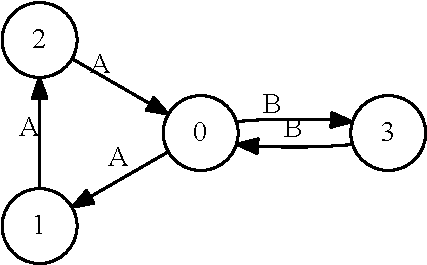
\includegraphics[width=6cm]{dot/input.pdf}
        \caption{Input graph $M$}
        \label{input}        
    \end{center}
\end{figure}

\begin{figure}[h]
    \begin{center}
        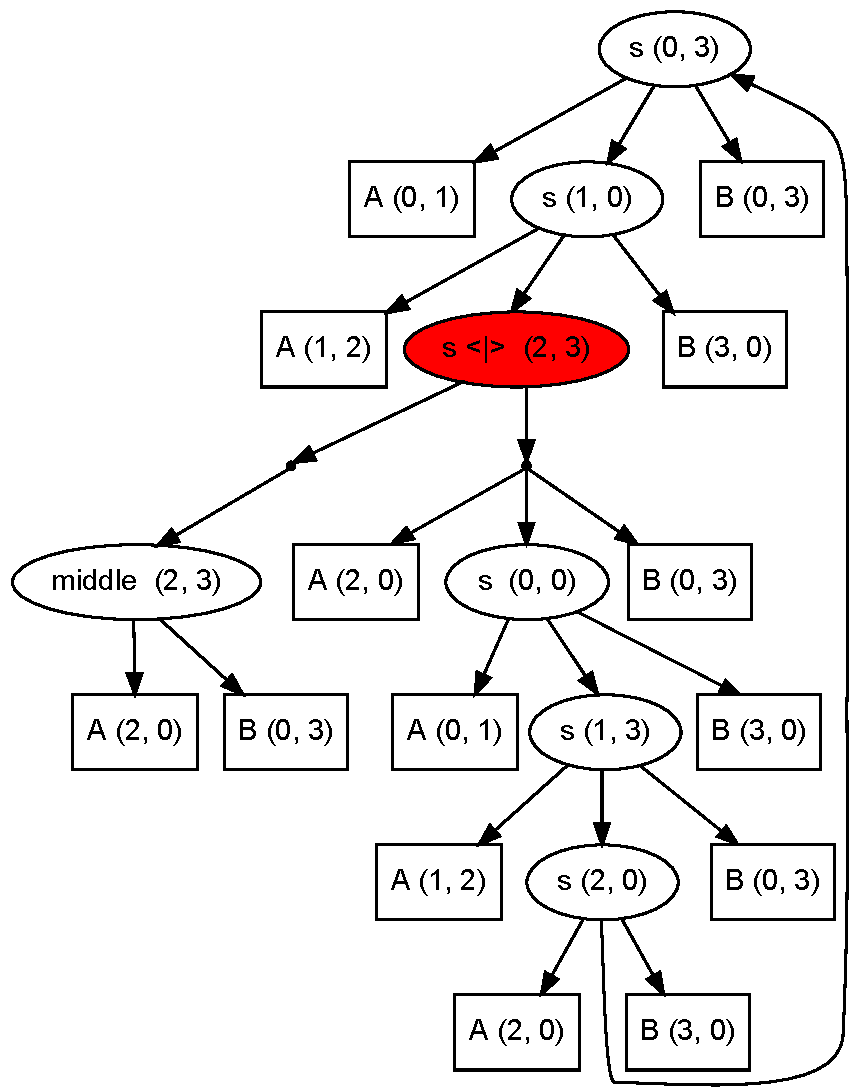
\includegraphics[width=9cm]{dot/AnBn.pdf}
        \caption{Result SPPF for input graph $M$(pic.~\ref{input}) and query $G$(pic.~\ref{grammarG})}
        \label{SPPF}        
    \end{center}
\end{figure}


\begin{thebibliography}{9}
  
\bibitem{DirOfBigGraphAnalysis}
Miller, J. A., Ramaswamy, L., Kochut, K. J., \& Fard, A. (2015, June). Research Directions for Big Data Graph Analytics. In 2015 IEEE International Congress on Big Data (pp. 785--794). IEEE.

\bibitem{FLCpathProblem}
Barrett, C., Jacob, R., \& Marathe, M. (2000). Formal-language-constrained path problems. SIAM Journal on Computing, 30(3), 809-837.

\bibitem{GLL}
Scott, E., \& Johnstone, A. (2010). GLL parsing. Electronic Notes in Theoretical Computer Science, 253(7), 177--189.

\bibitem{ConjCFPathQuery}
Hellings, J. (2014). Conjunctive context-free path queries.

\bibitem{PathQuerySemantic}
Hellings, J. (2015). Querying for Paths in Graphs using Context-Free Path Queries. arXiv preprint 
arXiv:1502.02242.

%\bibitem{CFPathQuery}
%Sevon, P., /& Eronen, L. (2008). Subgraph queries by context-free grammars. Journal of Integrative 
%Bioinformatics, 5(2), 100.

\end{thebibliography}

\end{document}
